%%%%%%%%%%%%%%%%%%%%%%%%%%%%%%%%%%%%%%%%%
% NIH Grant Proposal for the Specific Aims and Research Plan Sections
% LaTeX Template
% Version 1.0 (21/10/13)
%
% This template has been downloaded from:
% http://www.LaTeXTemplates.com
%
% Original author:
% Erick Tatro (erickttr@gmail.com) with modifications by:
% Vel (vel@latextemplates.com)
% Michael ma2196@columbia.edu
% with assistance from Jonah G.
% Adapted from:
% J. Hrabe (http://www.magalien.com/public/nih_grants_in_latex.html)
%
% License:
% CC BY-NC-SA 3.0 (http://creativecommons.org/licenses/by-nc-sa/3.0/)
%
%%%%%%%%%%%%%%%%%%%%%%%%%%%%%%%%%%%%%%%%%

%----------------------------------------------------------------------------------------
%	PACKAGES AND OTHER DOCUMENT CONFIGURATIONS
%----------------------------------------------------------------------------------------

\documentclass[11pt,notitlepage]{article}

% A note on fonts: As of 2013, NIH allows Georgia, Arial, Helvetica, and Palatino Linotype. LaTeX doesn't have Georgia or Arial built in; you can try to come up with your own solution if you wish to use those fonts. Here, Palatino & Helvetica are available, leave the font you want to use uncommented while commenting out the other one.

\usepackage{palatino} % Palatino font
%\usepackage{helvet} % Helvetica font
\renewcommand*\familydefault{\sfdefault} % Use the sans serif version of the font
\usepackage[T1]{fontenc}
\linespread{1.05} % A little extra line spread is better for the Palatino font

\usepackage{lipsum} % Used for inserting dummy 'Lorem ipsum' text into the template
\usepackage{amsfonts, amsmath, amsthm, amssymb} % For math fonts, symbols and environments
\usepackage{graphicx} % Required for including images
\usepackage{booktabs} % Top and bottom rules for table
\usepackage{wrapfig} % Allows in-line images
\usepackage[labelfont=footnotesize]{caption} % Make figure numbering in captions bold
\usepackage[top=0.5in,bottom=0.5in,left=0.5in,right=0.5in]{geometry} % Reduce the size of the margin
\pagestyle{empty} % Remove page numbers

\hyphenation{ionto-pho-re-tic iso-tro-pic fortran} % Specifies custom hyphenation points for words or words that shouldn't be hyphenated at all

  
  % to reduce white space between PARAGRAPHS
\setlength{\parskip}{0pt}
\setlength{\parsep}{0pt}

  % additional parameters
%\setlength{\headsep}{0pt}
%\setlength{\topskip}{0pt}
%\setlength{\topmargin}{0pt}
%\setlength{\topsep}{0pt}
%\setlength{\partopsep}{0pt}

  % to reduce white space around figures
% \setlength{\textfloatsep}{0pt plus 0pt minus 0pt}

  % to reduce white space between SECTIONS
\usepackage[compact]{titlesec}
\titlespacing{\part}{0pt}{5pt}{4pt}
%\titlespacing{\subsection}{0pt}{*0}{*0}
%\titlespacing{\subsubsection}{0pt}{*0}{*0}
%\titlespacing{\subparagraph}{0pt}{*0}{*0}
\titlespacing*{\subparagraph} {\parindent}{1ex plus 1ex minus .2ex}{0.5em}


\begin{document}


%----------------------------------------------------------------------------------------
%	SPECIFIC AIMS
%----------------------------------------------------------------------------------------
\part*{Specific Aims}
We propose to improve prediction and prevention of respiratory failure and death in hospitalized patients by integrating complex Bayesian hierarchical modeling into data imputation, patient triage and treatment implementation in electronic medical record based (EMR) surveillance.\newline
\textbf{Severe acute respiratory failure (ARF) requiring mechanical ventilation leads to increased mortality,} increased cognitive and functional impairment. EMR surveillance can identify hospitalized patients at risk, days before their deteriorating conditions are typically recognized; earlier initiation of preventive interventions can reduce morbidity, mortality and expenses: My mentor Dr. Gong is leading a two phase pragmatic trial: APPROVE, phase 1, develops a classical algorithm to identify patients at risk; PROOFCheck, phase 2, aims to improve outcomes by triggering an individualized prevention checklist for patients identified as at risk by APPROVE. \newline
\textbf{Our Bayesian model may outperform the classical prediction model thanks to partial pooling.} 
We propose to fit a more complex hierarchical Bayesian prediction algorithm, (1) by allowing model parameters to vary between patients, between medical floors, services or institutions and (2) by modeling temporal effects, e.g. institutional learning during trial implementation. We will outperform Dr. Gong's classical prediction algorithm by (a) partial pooling and (b) modeling the rich spatial and temporal organization of our electronic medical records more realistically: Patients treated by the same team, in similar settings will show similar clinical trajectories and responses. Especially in the subset with sparse or missing data, precision and accuracy of parameter estimates will be improved by partial pooling, because they are informed by data from all the other patients. 
\newline \textbf{Incomplete data limits prediction algorithms, poor compliance compromises effective interventions} and outcomes research. With my co-mentor Dr. Hall, I will advance Bayesian data imputation using auxiliary data, a novel approach to overcome issues with missing at random assumptions. Seasonal effects, changing population characteristics or provider behavior may limit prediction accuracy. We will update our model continuously with new patient information, adjust for seasonal effects and institutional learning. Last but not least, effective therapy only works if implemented; we will investigate what predicts provider compliance with our EMR-triggered alerts. 
\newline \textbf{Implementation of Bayesian hierarchical modeling can be computationally challenging for Big Data.} My co-mentor Dr. Gelman is leading the NSF-funded development of STAN. STAN's novel Hamiltonian Markov Chain Monte Carlo algorithm achieves much faster convergence and parameter estimation. With my exceptional and multidisciplinary team of mentors, I will integrate innovative approaches to data imputation with complex hierarchical prediction models to form a "real time" EMR-based clinical decision tool. We will overcome current limitations in Bayesian computational implementation for multi-center EMR-based outcomes research. This integration of pioneering statistical modeling with pragmatic EMR-surveillance constitutes the unique innovation of my proposal.

\begin{flushleft}
\textbf{Hypothesis:} \textit{Hierarchical Bayesian modeling compared to the classical model improves imputation, prediction, prevention and compliance analysis in a pragmatic trial to prevent respiratory failure in hospitalized patients.}
\end{flushleft}

\subsection*{Specific aims:}

\subsubsection*{Aim 1: To improve incomplete data imputation and early prediction of acute respiratory failure.}
\textbf{SA 1a:} To build a pragmatic EMR based hierarchical Bayesian model implemented in the ultra-fast statistical software Stan to predict a composite outcome [death or prolonged mechanical ventilation > 48 hours] in our Montefiore Medical Center inpatients and compare it with the existing classical (frequentist) algorithm. \newline \textbf{SA 1b:} To further develop Bayesian data imputation algorithms of missing clinical data using auxiliary data, to identify auxiliary measure properties (ceiling, floor and threshold effects), to integrate imputation and prediction in one coherent hierarchical Bayesian model and compare it to the classical algorithm by Dr. Gong.

\subsubsection*{Aim 2: To model temporality (institutional learning, seasons) and investigate provider compliance.}
\textbf{SA 2a:} To update our model continuously with new incoming patients to reflect their changing risk profile and to model institutional learning and temporal effects like seasons and endemics. 
\newline \textbf{SA 2b:} To investigate patient and provider characteristics as drivers of poor provider compliance in PROOFCheck, Dr. Gong's pragmatic trial, to inform the ongoing PROOFCheck trial implementation, refocus our retraining efforts and to explore the individualization of preventive interventions using EMR-context. 
%----------------------------------------------------------------------------------------
%	RESEARCH PLAN
%----------------------------------------------------------------------------------------
\newpage
\part*{Research Plan}

\section*{A. Significance}

\subsection*{Respiratory failure in hospitalized patients can be predicted and should be prevented.} 

\begin{wrapfigure}{R}{0pt}
 \vspace{-70pt}
 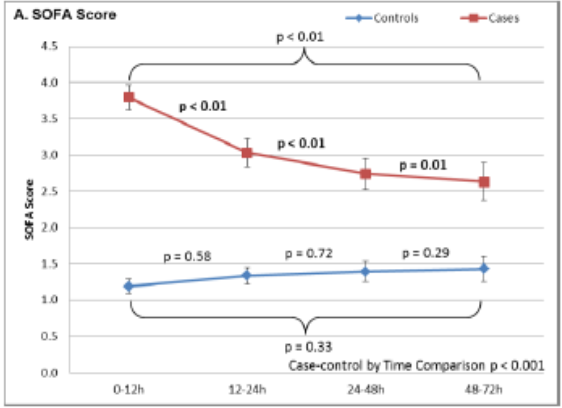
\includegraphics[scale=0.7]{Figures/SOFA_fig.png}
  \vspace{-30pt}
  \caption{\footnotesize Deterioration of the Sequential Organ Failure Assessment score (SOFA) can be detected 24 to 48 hours before clinical deterioration leads to ICU admission \cite{Yu_24970344}.}
    \label{fig:SOFA_fig}
 \vspace{-20pt}
\end{wrapfigure}

Acute respiratory failure requiring mechanical ventilation is common in hospitalized patients and consumes a disproportionate amount of health care resources in the United States \cite{Wunsch_20639743}. Short term mechanical ventilation can be live saving, but prolonged mechanical ventilation often leads to multi-organ failure and death in a third of patients \cite{Wunsch_20639743, Ranieri_10872010}.

Most research focuses on \textit{established} respiratory failure in the ICU, while detectable clinical signs and symptoms often herald the impending respiratory decompensation much earlier \cite{Rohde_23401431}. Dr. Gong co-developed the LIPS score to identify patients at high risk for the development of Adult Respiratory Distress Syndrome (ARDS) in the emergency department \cite{Herridge_12594312}, which proved equally able to discriminate the 587 patients in the cohort who progressed to severe ARF requiring > 48 hrs of mechanical ventilation. She also demonstrated that predictive scores deteriorate as early as 24-48 hours before ICU admission  [Figure~\ref{fig:SOFA_fig}] \cite{Yu_24970344}; but such ominous signs are either not recognized or not acted upon \cite{Hillman_12415452,McQuillan_9632403}. Early interventions (e.g appropriate antibiotic therapy, diuretics and chest physiotherapy) and preventive measures (e.g. head elevation) would be able to stop or reverse the clinical deterioration and/or prevent progression to multiple organ failure and prolonged mechanical ventilation or at least attenuate the subsequent clinical course \cite{Naeem_16150531,Rivers_11794169,Rivers_12594312,Mitchell_20378235}. 

\subparagraph{A pragmatic trials to predict and prevent mortality from respiratory failure in hospitalized patients.}  My mentor Dr. Gong is leading a NHLBI-funded multi-center cluster randomized pragmatic trial in two phases. (1) the first phase APPROVE aims to identify patients at risk by building classical logistic regression models based on electronic medical records (EMR) to Accurately Predict PROlonged Ventilation. (2) In the second phase PROOFCheck, identification of a patients at high risk triggers a decision support tool and bundled checklist of processes of care known to be beneficial in critically ill patients to PRevent Organ Failure. CITE CLINICAL TRIALS.GOV. The hypothesis is that for the patients identified as at high risk for prolonged respiratory failure or death in APPROVE, the early implementation of a checklist of preventive measure (PROOFcheck), reduces severity of organ failure, mortality and duration of mechanical ventilation. 

\subparagraph{Electronic medical records are an eminent example of richly structured and correlated Big Data} 
and hold enormous promise for outcomes research \cite{Dean_19279318,Amarasingham20940649},  exemplified by Dr. Gong's pragmatic trial. However, large electronic medical data sets are not just bigger in that there are more instances of the same thing, (e.g. more patients would make data analysis only easier).  Rather, there is more breadth to the data, and in the case of pragmatic trials, more heterogeneity, more subgroups, locations, or time granularity than is currently being modeled, more frequent and detailed measurements than can easily be incorporated into classical models.  This currently limits the scientific hypotheses and clinical inferences, that can be explored and evaluated. In Dr. Gong's pragmatic trial in particular, we desire more fine-grained information on the predictions to individualize prevention.  

\paragraph*{We can individualize prevention targeting patients at risk.}
Preventive measure, for example goal targeted resuscitation, decrease respiratory failure requiring mechanical ventilation, when they are initiated early \cite{Rivers_12594312}. However, an indiscriminate approach to prevention of respiratory failure in hospitalized patients will be ineffective, because only one in 30 hospitalized adults requires mechanical ventilation. Secondly, individualizing preventive and therapeutic measures specifically based on patient characteristics will be more efficient in preventing potentially irreversible end organ damage, while also  leading to improved compliance by providers and cost effectiveness. So how can we improve and individualize prediction and prevention? 

\subparagraph{Observations and outcomes in our pragmatic PROOFcheck trial will be nested hierarchically.}
For example, repeated oxygen saturation measurements will be similar in the same patients, the more so, the closer they are in time. Patients seen by one and same hospitalist in our system will tend to have similar outcomes, predicted by that physician's behavior and qualities. As an example, some physicians or services will follow a more liberal fluid management, others will emphasize early diureses; clearly this choice will summarily affect the respiratory failure risk of specifically those patients under this service or physician's care. Generally, physicians in academic medical centers like ours are organized in services, which are integrated across wards, clustered in hospitals. Concretely, the observations in our hospitalized patient cohort at Montefiore Medical Center, their outcomes and their propensity to respond to treatments, all are hierarchically nested; this requires more than just fitting well-known models at larger scales; richer models can exploit this fine-grained multilevel structures for optimal prediction of acute respiratory failure in our trial cohort. Finally, differences in regional health care environments predict patient, provider and institutional behavior and consequently outcomes, therefore risk patterns in one institution or even one region may not translate well to others; adjustments are surely necessary to translate our algorithms to different ecological settings. 

\subsection*{Bayesian hierarchical modeling is transformative for EMR based prediction.}

\begin{wrapfigure}{R}{5cm} % Example figure with text wrapping around it
 \vspace{-20pt}
 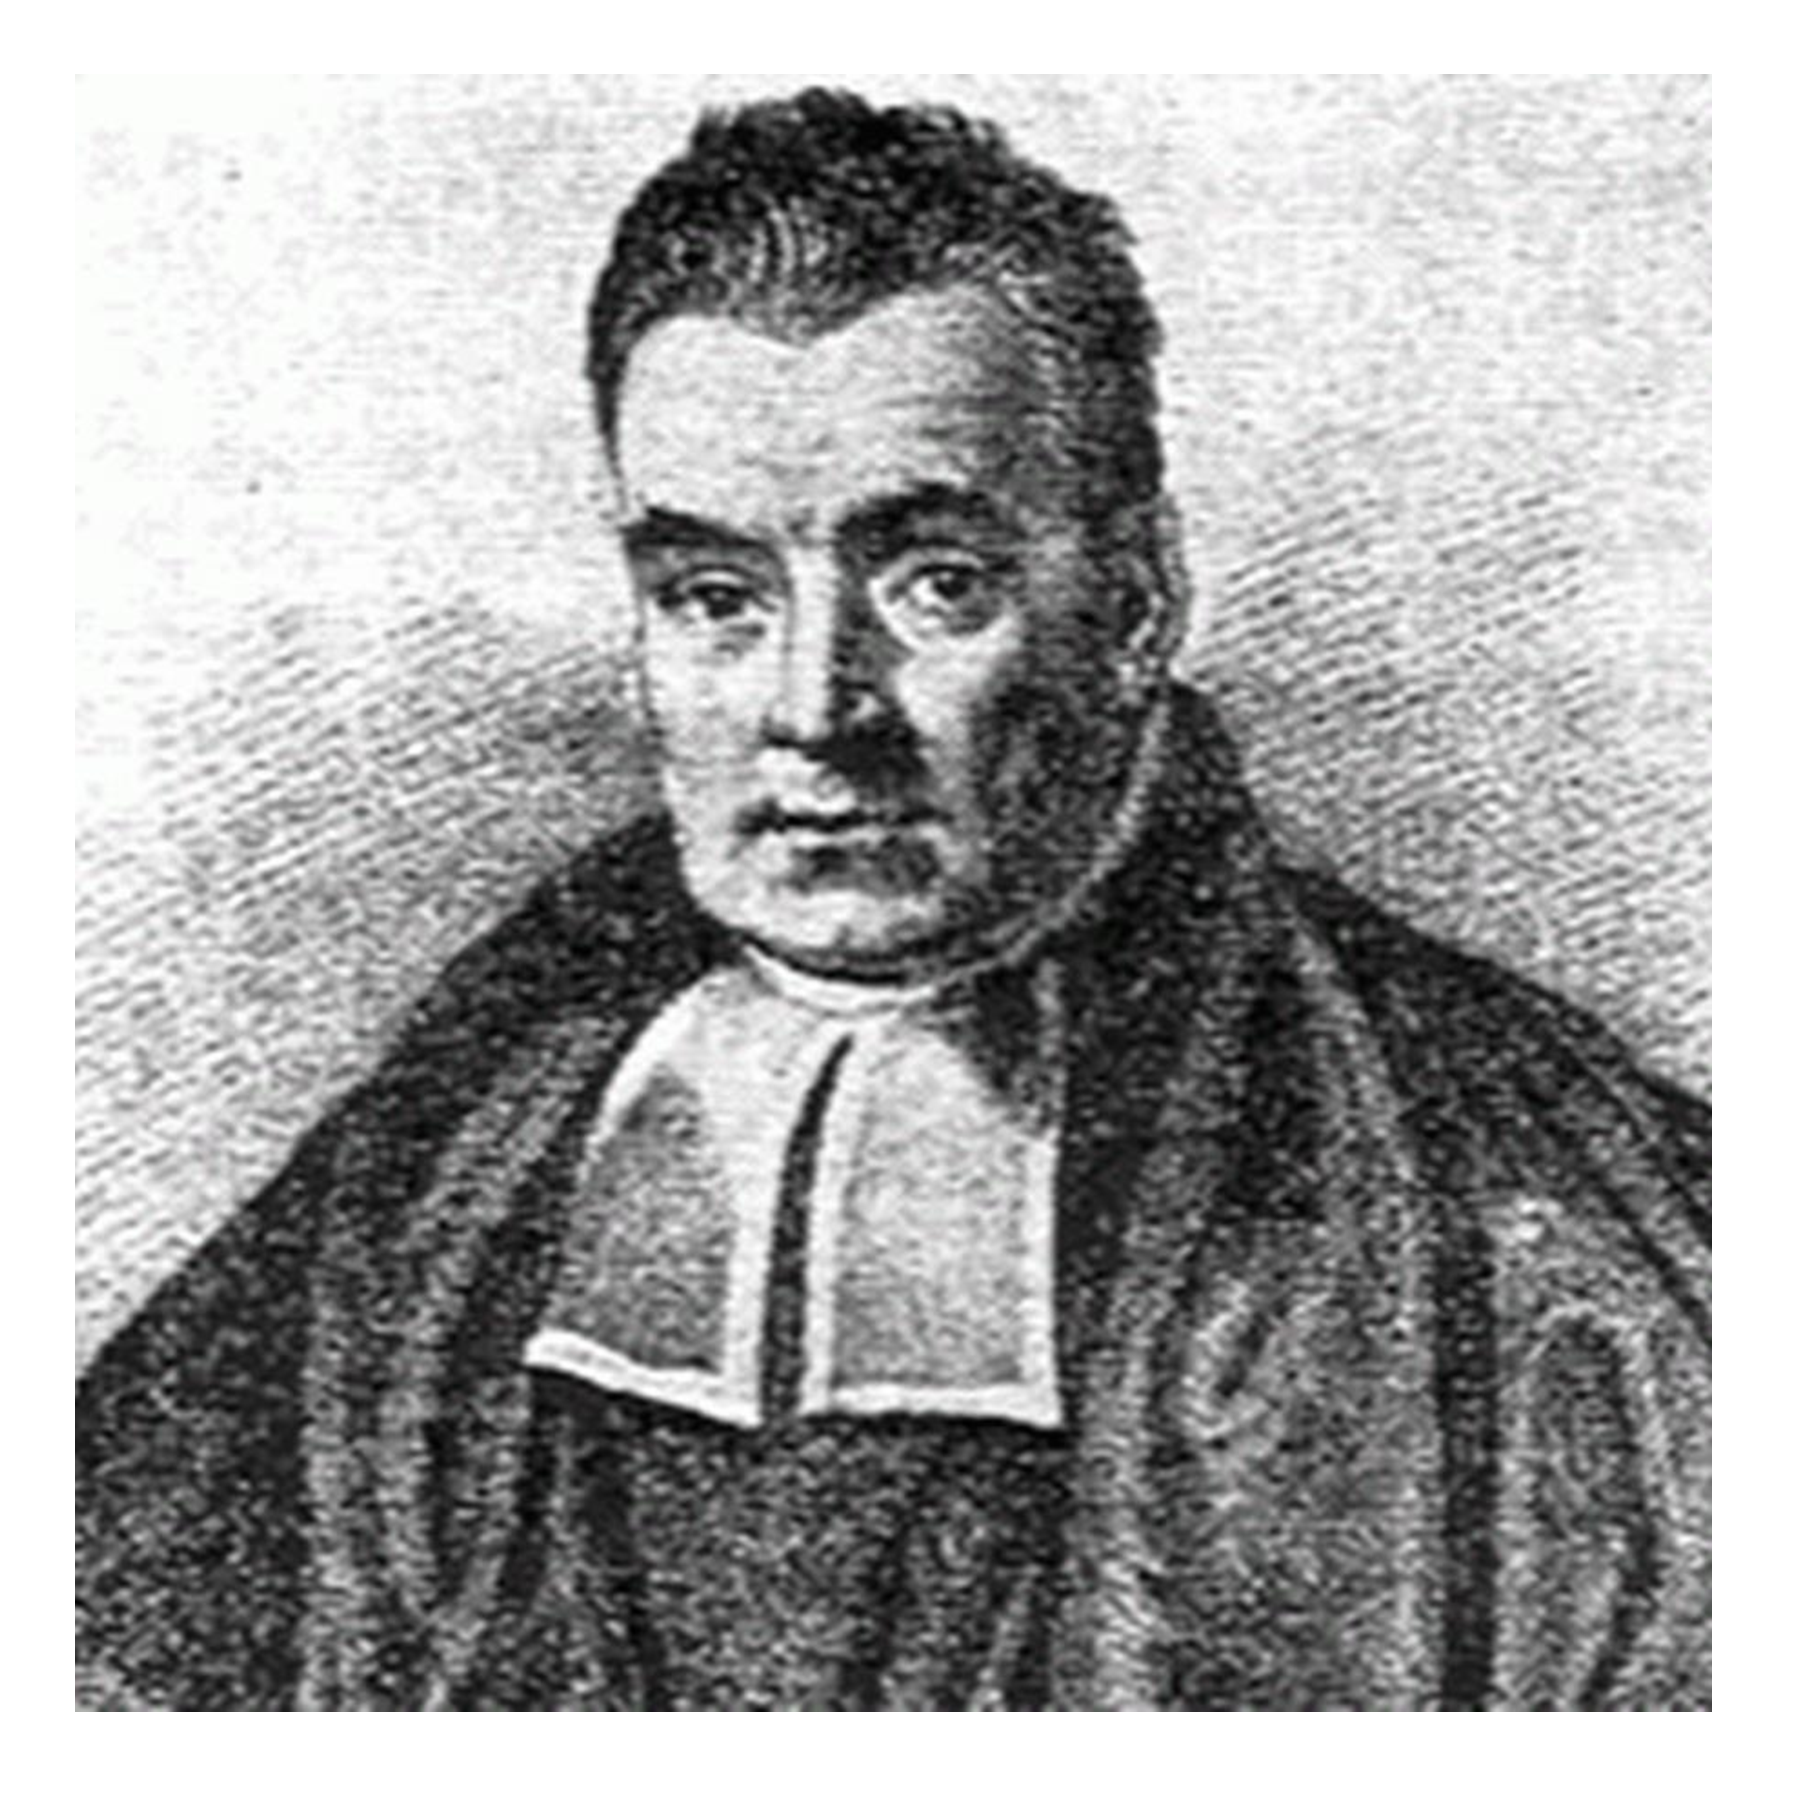
\includegraphics[scale=0.15]{Figures/Thomas_Bayes.pdf}
  \vspace{-10pt}
 \caption{\footnotesize Thomas Bayes formulated the Bayes Theorem, published in a posthumous paper in 1763. \cite{Thomas_Bayes}.}
 \vspace{-20pt}
\end{wrapfigure} 

\subparagraph*{Bayesian methods are old, but novel in EMR surveillance.}
Reverend Thomas Bayes (Portrait in Fig.1)\cite{Thomas_Bayes} formulated the Bayes theorem already in 1763 as an alternative statistical model. With a well developed theory, Bayesian methods are only novel in so far as they were rarely used in medical research until computers and Markov Chain Monte Carlo algorithms became widely available in the 1990s, leading to an expansion of applied Bayesian work \cite{Ashby_16947924,Spiegelhalter_11134920}, more recently also in Big Data \cite{Yoo_24987556}. Past constraints in computational implementation have largely been overcome, except maybe for very large complex data sets like EMRs. We are not aware of any Bayesian hierarchical prediction model based on large EMRs to date. However, now ultra-fast Hamiltonian Monte Carlo algorithms \cite{Stan_Software_2014} and clever statistical formulation or transformation allow to push the boundaries of computability, also for very large EMR data sets \cite{Gelman-Hill_2014}.  

\subparagraph*{A too brief introduction to Bayesian inference and its computational implementation.}
In Bayesian inference, prior information is combined with new data to yield an updated posterior estimate for the probability of a hypothesis \cite{Kruschke_Book_2014}. The Bayesian approach is hence analogous to clinical decision-making \cite{Spiegelhalter_11134920}. Physicians continuously update their preliminary diagnosis as new information comes in. Prior belief in a diagnosis may be weakened by new laboratory information, leading to an alternative disease hypothesis; or new lab information may reaffirm the initial diagnosis. \cite{Kruschke_22774788}. Bayesian methods are particularly suited for flexible hierarchical modeling \cite{Carlin_1349763,Sutton_2012}. 

Bayesian inference for more complex (hierarchical) models can often not be derived analytically; instead we calculate numerical approximations of the multi-dimensional integrals to obtain the posterior distributions of the parameters of interest. In technical terms, Markov Chain Monte Carlo (MCMC) based Bayesian inference methods sample from a posterior probability distribution after building a Markov chain. In lay terms, MCMC simulation replaces intractable analytical integration with empirical summaries of samples from the posterior distribution \cite{Abrams_9483729}: Instead of analyzing the odds, we simulate throwing the dice repeatedly. 

\subparagraph{Hierarchical modeling exploits the richly organized heterogeneity of electronic medical records.}
With their inherent flexibility and robustness, Bayesian hierarchical models may outperform classical models for prediction in large EMR data sets with spatial and temporal organization \cite{Gelman_red_2009}. Above we described our multilevel EMR, consisting of repeated visits by patients with different medical plans, ages and medical conditions, treated by different services integrated in different wards and hospitals. Fitting our predictive regression model, we would want the regression coefficients to vary by group (by service, by medical unit, by hospital), to realistically model the complex correlations seen in actual clinical practice: The number of parameters to estimate grows very quickly and so do the potential interactions. Reciprocally, even with very large data sets, the sample size in each subgroup will shrink rapidly; estimates using least squares or maximum likelihood will become noisy and thus often become essentially useless. One solution lies in hierarchical modeling, where we estimate hyper-parameters and hyper-hyper-parameters, to represent how lower level parameters vary across different groupings \cite{Bafumi_Gelman_2007}.

\subparagraph*{Prediction based on "partial pooling" outperforms the no-pooling and complete-pooling approach.}
Employing hierarchical modeling for our prediction model will be more efficient, as can be shown mathematically or via cross-validation \cite{Gelman-Hill_2014}. "No pooling" would be an alternative approach to estimate the model for each specific subset of interest separately. But addressing and exploring the complexity and granularity, the richness of the EMR data would lead to far too many sub-classifications, thus too small samples in any given subgroup for useful inferences. "Complete pooling" or structural modeling constitutes the other extreme of the spectrum, but the implied hard constraints on the coefficients in different groups may lead to bias: we loose information, because we cannot learn from groups where we have more data. We choose the middle ground: Prediction using "partial pooling" or hierarchical modeling is especially effective for our richly organized EMR data, because the estimate of each individual parameter is simultaneously informed by data from all the other patients in our cohort, improving prediction in particular for subgroups with sparse data \cite{Gelman_multilevel_2006}. \newline

\emph{We hypothesize that Bayesian hierarchical modeling may better identify hospitalized patients at risk for acute respiratory failure and prolonged mechanical ventilation than classical prediction algorithms.}


\subparagraph*{Heterogeneous and incomplete clinical data may limit prediction and implementation.}
Variables with strong predictive power in our model may not be recorded in all patients or may be missing for the time window needed for prediction, limiting development of the prediction algorithm, implementation of the therapeutic interventions and the trial itself. To improve prediction for cases with incomplete data, we can impute the missing data. Informative loss by non-ignorable incomplete data may bias risk prediction or may hamper the implementation of the prediction algorithm. Likelihood-based mixed effects models for incomplete data give valid estimates if and only if the data are ignorably missing; that is, the parameters for the missing data process are distinct from those of the main model for the outcome, and the data are missing at random (MAR) \cite{Rubin_1976}. However, this is an unreasonable assumption for our electronic medical records, for example because physicians will request test based on the patients co-morbidity and current clinical conditions. Data will not be missing at random, instead incomplete data will be associated with predictors and outcomes; this could lead to biased imputations.

\subparagraph*{Auxiliary data can be used to impute incomplete medical records.}
Auxiliary date are additional information available in the form of variables known to be correlated with the missing data of interest \cite{Daniels24571539}. In our data set we find that arterial blood gas oxygen tension is often unavailable for the prediction time window, because it was not requested by the physicians. In this case peripheral oxygen saturation and or or oxygen therapy may be used to impute the peripheral arterial blood oxygen tension [Figure~\ref{fig:Imputation_fig}]. This approach avoids the perils associated with missing at random (MAR) assumptions, when fitting a non-ignorable missingness model \cite{Wang_20029935}. Adding auxiliary variables not included in the main model for multiple imputation, in other words using additional information that is correlated with the missing outcome is an emerging approach to help correct bias \cite{Meng_1994, Collins_11778676, Rubin_1996}, often relying on Bayesian methods for the multiple imputations approach \cite{Daniels_2008, Schafer_1997}; joint modeling and multiple imputations could both be used also to impute incomplete medical records \cite{Fitzmaurice_2008}. The use of auxiliary data to impute incomplete patient records will improve the prediction model and facilitate smoother implementation of the algorithm into the clinical trial \cite{Hall_25389642}. Moreover, auxiliary data imputation for incomplete electronic medical records is underdeveloped; methodologically, their development is an innovative hallmark of this proposal.

\subparagraph*{Seasonal effects and institutional learning can bias risk prediction and can thwart implementation} or imperil the effectiveness of our efforts to mitigate the risks of severe respiratory failure in hospitalized patients. Like for any institution, the composition of the Montefiore Medical Center population, their co-morbidities and risk profiles change over time, altering which patient characteristics best predict severe adverse respiratory failure and mechanical ventilation. More importantly, we noted during the implementation phase of previous preventive trials, that providers learn, changing their behavior as a result of trial participation. As trials progressed providers implemented previously underutilized interventions more frequently even before they were prompted. We term this effect institutional learning. The transition of junior and senior providers through their training and to other institutions and new personnel joining the staff, may on the other hand led to these improvements being lost. Last but not least, respiratory disease is affected by seasonal and secular effects; influenza prevalence for example is seasonal and characterized by major and minor epidemics. Seasons and epidemics will affect the predictive power of any model and hence also alter the risk profile of our patients over time. Institutional culture and individual provider behavior change in response to trials and quality improvements interventions; patient populations change over time. Respiratory patients are plagued by seasonal deterioration. These temporal, seasonal and secular effects will alter the predictors of risk in our model and affect its implementation. We will therefore include institutional learning, seasonal effects and continuously update our model with new patient data to account for said changes in the risk profile. The integration of institutional learning, secular and seasonal effects in a EMR-triggered prediction and prevention within one coherent (Bayesian) model is novel. 

\subsection*{Analyzing and advancing implementation is decisive for outcome improvement and research.}

\subparagraph*{Imperfect fidelity (poor provider compliance) is a major concern also in our PROOFcheck trial,} just as non-compliance is a major obstacle to the effective delivery of health care and improved outcomes in general
\cite{Duncan_16710766}. The targeted interventions triggered by our EMR-prediction algorithm will only prevent respiratory failure if our physicians and nurses actually implement them. Improving fidelity of health care providers with evidence based interventions continues to be a challenge and is under-researched \cite{Davis_7650822} and little is known on how to reproducing complex interventions (specially directed toward providers) to improve clinical outcomes \cite{Campbell_10987780}. As long as we do not understand what drives provider fidelity and patient compliance with the preventive measures proposed to our providers for their high risk patients  \cite{Mittman_15172904}, we ignore the best means to translate widely accepted interventions and new findings of outcomes research into practice \cite{Glasgow_17150029}. We need to understand better what patient and/or provider characteristics hinder compliance with the triggered preventive checklist interventions to ensure care is in accordance with accepted evidence based best practices.

\subparagraph*{We use a pragmatic trial to investigate heterogeneous provider fidelity with in clinical implementation.} Pragmatic trials like Dr. Gong's may result in valid estimates of effectiveness in more realistic health care scenarios \cite{Selby_22824225,Tosh_21842618}; we will use her pragmatic trial data to investigate incomplete fidelity, heterogeneity and difficulty in clinical implementation. An example with problematic fidelity relevant for PROOFcheck is blood product management; transfusions increase the risk of acute severe respiratory failure with mechanical ventilation \cite{Kenz_24892308};  recent research led to consensus that overzealous and empiric transfusion of blood products leads to worse outcomes \cite{Hebert_9971864}, acknowledging that untreated anemia also predicts poor outcome \cite{Ranucci_22698773}; guidelines reflect this for over a decade \cite{ASA_25545654}, but  years later, implementation of rational transfusion blood product management is sketchy and very heterogeneous across the nation \cite{Likosky_20488928}; not least because their complex algorithms can be difficult to follow. Weiss et al. demonstrated that direct prompting for best practices improves provider compliance in the ICU and outcomes such as duration of mechanical ventilation or length of stay \cite{Weiss_21616996}. We hypothesize that fidelity will be associated with certain provider and patient characteristics; their investigation will allow more focused re-education efforts and adaptation of the checklist implementation. 

\section*{B. Innovation}
\subparagraph*{Focus on prevention of critical adverse outcomes in hospitalized patients.}
Changes in reimbursement give providers a stake in patient outcomes and led to a keen interest in the prediction and prevention of adverse event in hospitalized patients. It makes sense to focus early intervention on patients at high risk for poor outcomes. This project advances hierarchical Bayesian models to implement this paradigm shift in very large electronic medical records, triggering personalized interventions that drive outcome improvements. This is novel and has not been attempted to our knowledge.

\subparagraph*{Improve imputation of incomplete electronic medical records.}
Incomplete patient data, typical for actual clinical records can hinder the development and execution of our prediction algorithms and implementation of the pragmatic trial. We will further Bayesian methods to impute incomplete missing data from additional auxiliary data to overcome this limitation. Beyond improving prediction and patient outcomes in our clinical trial, the Bayesian methods we propose to develop can be employed to impute incomplete electronic medical records in other settings.

\subparagraph{Analyzing and understanding the drivers of poor provider compliance} in a multicenter pragmatic trial like Dr. Gong's will be important for any EMR-based outcomes research or quality improvement, and will have implications beyond for any clinical trial, indeed for clinical practice at large.

\subparagraph*{Integrate advances in critical care with cutting edge computational statistics.}
To often advances in statistical modeling and clinical science are worlds apart. We want to address a critical problem of scalability in Big Data inference, but are equally motivated by our practical use case, improving our pragmatic clinical trial. The strength of our proposal, therefore, is the integration of disparate disciplines, critical care and computational statistics. 

\subsection*{Summary of the impact}
We tackle a serious health care challenge by integrating advanced hierarchical modeling into a pragmatic clinical trial. Beyond improving morbidity and mortality from respiratory disease in hospitalized patients through improved prediction and prevention, we will develop new methods to impute incomplete electronic medical records from auxiliary data and scale Bayesian hierarchical models to use in large EMR data and will investigate drivers of poor provider compliance. Our proposal is unique and novel in its integration of cutting edge methods from clinical, statistical and computer science to fully realize the promise of Big Data in critical care.

\section*{C. Approach}
My research project will be closely aligned with my mentor's NIH-funded pragmatic two phase trial. Aim 1 will utilize the processed data of APPROVE to improve the prediction model and Aim 2 will use the data from the implementation of PROOFcheck to investigate fidelity of the providers with the EMR-triggered interventions.

\subsubsection*{Aim 1: To improve early prediction of prolonged respiratory failure and death in hospitalized patients.}

\begin{flushleft}
\textit{Hypothesis: Our hypothesis is that the integration of complex hierarchical Bayesian modeling and data imputation will improve prediction of severe respiratory failure in hospitalized patients compared to the classical statistical approach.}
\end{flushleft}

\begin{wraptable}{r}{4.8cm} % Example table with text wrapping around it
\caption{Table describing the population?}
\begin{center}
\begin{tabular}{l l r}
\toprule
\multicolumn{1}{c}{City} & {N\textsuperscript{a}} & {\%Silly}\\
\midrule
San Diego & 289 & 41\%\\
Seattle & 262 & 32\%\\
Galveston & 261 & 15\%\\
St Louis & 269 & 7\%\\
New York & 271 & 4\%\\
Baltimore & 231 & 2\%\\
\emph{Total} & 1,586 & 21\%\\
\hline
\end{tabular}\\
\footnotesize\textsuperscript{a}{Inpatient population at Montefiore Medical Center.}
\end{center}
\label{default}
\end{wraptable}

\subparagraph*{For specific aim 1a,} we will build a pragmatic EMR-based hierarchical Bayesian model to predict a composite outcome [mechanical ventilation prolonged beyond 48 hours or death] in hospitalized adult and compare our Bayesian approach with the existing frequentist algorithm used by Dr. Gong in her pragmatic trial.

\subparagraph*{Population:}
We will include all adults patients, admitted to the Montefiore Medical Center during the study period, excluding only those who are chronically ventilated at home or who have Do not resuscitate orders at the time of hospital admission (Table 1: Inpatient population at Montefiore Medical Center.) As part of APPROVE, the pragmatic trial by Dr. Gong described in detail under Significance, two 3-month, prospective, observational cohort studies are underway at several Albert Einstein College of medicine and Mayo Clinic Rochester and Florida sites; we will build our Bayesian hierarchical model based solely on Einstein patients: Patients from the first three months will serve as the fitting cohort, while the 2nd cohort will serve as the validation and test set.  

\subparagraph*{Predictors:}
Many independent variables are candidates for potential inclusion into our Bayesian hierarchical model. From the multicenter LIPS study, clinical factors most closely associated with prolonged mechanical ventilation have already been identified \cite{Herridge_12594312}. We will consider these and additional time-invariant and time-variant demographic and clinical data. Examples for demographics are gender, age, medical service or ward, examples for physiological and clinical predictors are heart rate, blood pressure or lab tests, respectively. Certain predictors will require summary aggregations and (logarithmic) transformations to induce variance stability.

\subparagraph*{Outcomes:}
Our primary dichotomous outcome will be acute respiratory failure requiring mechanical ventilation longer than 48 hours. Outcomes are specified as positive for a) mechanical ventilation lasting longer than 48 hours or b) mechanical ventilation lasts less than 48 hours, but the patient died within 96 hours of the calculated score. Patients that are not on prolonged ventilation within 96 hours or discharged alive from the hospital will be considered negative.

\subsubsection*{Bayesian hierarchical modeling to reflect the nested structure of health care}
We will build a Bayesian hierarchical multivariate logistic regression model of time-invariant and time-variant demographic, clinical and administrative variables. Our Bayesian hierarchical modeling will represent the multi-level nested structure of current health care, with levels for medical or surgical service the patient is under, the floor or ward where the patient is cared for, the institution the patient is admitted to. We will also consider other random effects for example for co-morbidity and other time-invariant patient specific descriptors. We illustrate this nested structure in a simple logistic model with hierarchical levels for patient, service and hospital: 

\subparagraph*{Patient level}
At the patient level, we may model the probability $alpha$ that a patient will develop the dichotomous event $Y$, acute respiratory failure requiring mechanical ventilation, using arterial oxygen tension $PaO_{2}$ as a predictor in a simple logistic regression model: 
\begin{align}
Y \sim Binom (\alpha, n) \\
\alpha = inv_log (\beta_{0} +\beta_{1} * PaO_2)
\end{align}

\subparagraph*{Service  level}
Patients are typically assigned to hospital services. Pulmonary service patients may have a lower baseline $PaO_2$. Surgical patients tend to have normal lung function. Hence we may model $\beta_{0}$ to allow different intercepts representing the average $PaO_2$ of patients in the various medical and surgical services estimating different service level mean intercepts $\gamma_0$. Under a medical service, smaller changes in $PaO_2$ may be indicative of respiratory deterioration compared to a surgical service, where larger drop in arterial oxygen tension predicts outcome. We may hence allow the regression coefficient for the slope $\beta_{1}$ to vary around different mean slopes $\gamma_1$ at the service level : 
\begin{align}
 \beta_{0} \sim Normal (\gamma_0 , \tau_{\beta_0}) \\
 \beta_{1} \sim Normal (\gamma_1, \tau_{\beta_1})
\end{align}

\subparagraph*{Hospital level}
Some hospitals may cater to an economically disadvantages population, which is sicker on average. To reflect this, we may  model the mean intercept $\gamma_0$ for the services hierarchically at the hospital level. Some hospitals are organized such that patients differ very much between services, other hospitals may have a more homogeneous patient distribution; this \textit{variation} $\tau_{\beta_1}$ of the mean slope $\gamma_1$ within services at a given hospital can also be modeled to capture the variability of the predictive effect of lower $PaO_2$:
\begin{align}
\gamma_0 \sim Normal (\delta, \zeta) \\
\tau_{\beta_1} \sim Normal(\delta_tau, \kappa) 
\end{align}

\subparagraph*{APPROVE is the compared frequentist prediction model}
Dr. Gong's statistical team will build employing the published LIPS score \cite{Herridge_12594312} to identify hospitalized patients at risk for prolonged mechanical ventilation and death. The score at the selected start time will be used to determine the best cutoff score to identify the patients with the highest risk of developing prolonged mechanical ventilation.

\begin{wrapfigure}{R}{0pt}
 \vspace{-70pt}
 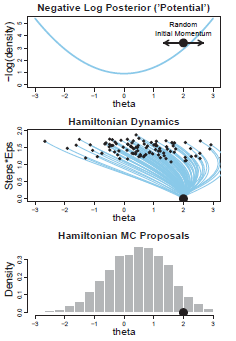
\includegraphics[scale=1]{Figures/Hamiltonian.png}
  \vspace{-30pt}
  \caption{\footnotesize Hamiltonian MCMC uses momentum to optimize the next proposal. The higher momentum of the current position (black dot) is indicated in the top panel. The middle panel illustrates how random samples are drawn to the mode of the posterior distribution (lower panel) leading to faster convergence and higher effective sample size. Fig 14.1 in Kruschke \cite{Kruschke_Book_2014}.}
    \label{fig:Hamiltonian}
 \vspace{- 15 pt}
\end{wrapfigure}

\subparagraph*{Data Acquisition}
Data will be abstracted from a clinical data warehouse(see Environment and Resources). A multi-prong approach for capturing complete, longitudinal data in real-time, near real-time, or asynchronously from the EMR replica will be used. When possible, and where collection of additional complementary information is warranted, we will use the Retrieve Form for Data Capture IS THIS THE CORRECT REFERENCE?\cite{Rothenhaeusler_2005},an IHE30 IS THIS THE CORRECT REFERENCE? \cite{Rotte_15809512} standard for gathering new data within a user's current application environment (EMR in this case) to meet the requirements of an external system. Secured electronic data capture tools provided by the Montefiore Enterprise Clinical Research Management System will be used to streamline, quality control, normalize, and manage data collection and data entry efforts. A fully de-identified, study specific database of all study variables will be compiled for model development and validation. When subsequently patient data from additional regional medical centers are incorporated, site identifier variables will be obfuscated to blind investigators.

\subparagraph*{Computational Implementation:}
We will implement the Bayesian model in the ultra-fast probabilistic programming language software STAN developed by my co-mentor Dr. Gelman \cite{Stan_Software_2014}. Clever statistical transformations to sample in the standardized normal space will take full advantage of the faster convergence and higher effective sample size of STAN and overcome computational limitations of Bayesian hierarchical models for Big Data \cite{Gelman-Hill_2014}. STAN  is based on Hamiltonian Monte Carlo (HMC) \cite{Gelman-Hill_2014}, a Marcov chain Monte Carlo (MCMC) algorithm, which avoids the sensitivity to correlated parameters that plague many MCMC methods by introducing auxiliary momentum variables \cite{Homan_Gelman_NUTS_2014} as illustrated in Figure~\ref{fig:Hamiltonian}. HMC is dependent  on tuning the reciprocal relationship of the crucial parameters step size and desired number of steps. If the latter is too large, efficiency is low, if to small we see undesirable random walk behavior. To overcome this, STAN implemented the No-U-Turn Sampler (NUTS), a recursive algorithm to automate and optimize tuning the HMC \cite{Homan_Gelman_NUTS_2014}, also introduced by my co-mentor Dr. Gelman. If needed, we will run chains in parallel on Columbia Univ.'s mainframe computer cluster. 

\subparagraph*{Posterior predictive checking, predictive validations and model comparison}
In evaluating its predictive performance, we will perform exploratory graphical \cite{Gelman2004posteriorpredictivechecks} and confirmatory formal posterior predictive assessment using discrepancies \cite{GelmanMengStern1996} to compare the patient test set to simulated replications from our fitted hierarchical Bayesian model, predictive validation to adjust for overfitting of our model and a sensitivity analysis of our priors on key model parameteters \cite{Gelman-Hill_2014,Gelman_predictive_2000}. We will compare our Bayesian Model to the frequentist algorithms using the minimum $\chi^{2}$ discrepancy, essentially equivalent to the classical
goodness-of-fit test statistic \cite{GelmanMengStern1996}. For additional validation and as a safeguard against over-fitting, we will train our model with patient data from other participating institutions (Mayo Clinic Rochester and Florida) and test if our model outperforms the classical prediction models even in other ecological settings, both if the classical frequentist model is based on data from all institutions or the test institution (say Mayo Clinic Rochester) alone.

We will compare models by parallel sampling \cite{Congdon_modelcomparison_2005}

\subparagraph*{Technical approach}
Boolean combinations of data matching and natural language processing of the prediction algorithms will be used to scan a real time copy of the hospital's clinical and administrative data including demographic, monitoring, pharmacy, laboratory, and physician notes for risk factors and physiological abnormality. Figure~\ref{fig:implementation} illustrates the implementation algorithm. The rule engine (implemented in Java) will send out the alert to providers.
We will integrate Bayesian patient triage into the infrastructure established during PROOFcheck, Dr. Gong's pragmatic trial, if we can show that our Bayesian prediction algorithm is superior to the existing algorithm. Based on our analysis for aim 2, compliance information will be reviewed for various items during the course of study so that sites could be targeted for re-education.

\subparagraph{Exploratory analysis}
As an exploratory analysis, we will investigate if a score deterioration over time (even less than the cut off for high risk,) improves prediction, in particular if it reduces false negative rates, in which case we shall incorporate it into our prediction algorithm.

\subsubsection*{We will advance Bayesian incomplete EMR-data imputation using auxiliary data}
Missing data are a characteristic limitation of large electronic medical records and may bias our prediction model \cite{Dean_19279318}. Electronically medical records measurements not updated 24 hours earlier than the selected start time will be considered missing;  


\begin{wrapfigure}{R}{10cm} 
 \vspace{-30pt}
 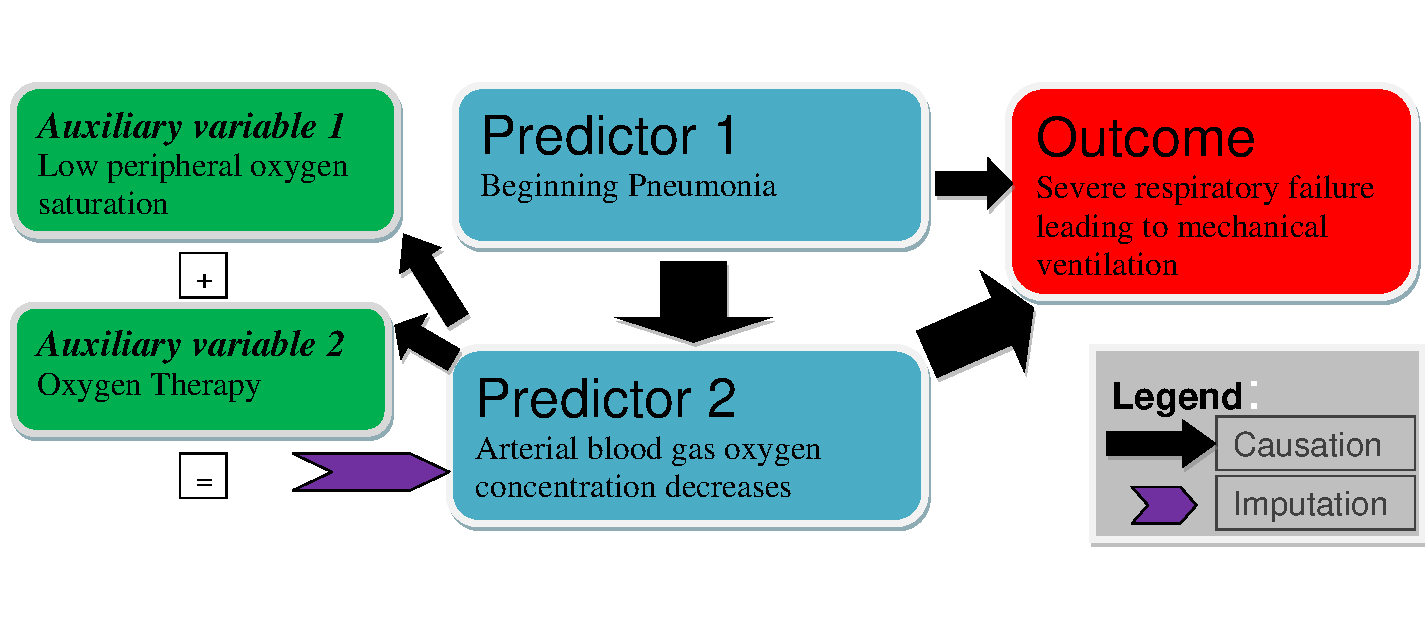
\includegraphics[scale=0.4]{Figures/Bayesian_imputation.pdf}
    \vspace{-20pt}
  \caption{\footnotesize Incomplete data can hinder outcome prediction, but we can impute incomplete data from auxilliary information. For example, pneumonia (causing to low oxygen tension), may cause respiratory failure. If arterial blood gas results are missing, we can impute the oxygen tension from oxygen therapy and/or peripheral oxygen saturation. \cite{Hall_25389642}.}
   \vspace{-20pt}
    \label{fig:Imputation_fig}
\end{wrapfigure}

\subparagraph{}
As an illustrative example, we formulate a simplistic model illustrated in [Figure~\ref{fig:Imputation_fig}]. We combine the prediction of the dichotomous compound outcome $Y$,(defined as acute respiratory failure leading to mechanical ventilation and death) using latent arterial oxygen tension $\Omega$ in a logistic regression model. 
\begin{align}
Y \sim Binom(\mu, n) \\
\mu = inv\_log(\beta_{0} + \beta_{1} * \Omega)
\end{align} 
We may have the $PaO_{2}$ from an arterial blood gas (ABG) or not. Nota bene, ABGs will certainly not be missing at random, but contingent on the $PaO_2$ value and respiratory outcome $Y$. If the $PaO_{2}$ from the ABG is observed, we will use it to predict the outcome $Y$. If no ABG was obtained, we impute the latent aterial oxygen tension $\Omega$ with a regression model from the auxiliary data  $O_{2}$ Saturation and $O_{2}$ therapy, formally:
\begin{align}
\Omega =  I(observed = true) * PaO_{2}   +   I(observed = false) * \delta  \\ 
\delta \sim Normal(\theta, \tau), 
\theta = \gamma_{0} + \gamma_{1}* O_{2} Sat + \gamma_{2} * O_{2} Therapy
\end{align}
We will exploit the temporal relationship between variables in the longitudinal electronic medical records \cite{Welch24782349}. We will identify the auxiliary measure properties, ceiling and floor and potential threshold effects effects, test the imputations against manually verified data and published algorithms and compare them to the simple and multiple imputation strategies planned for Dr. Gong's pragmatic trial \cite{Huntington_16311133,Sloan_15027501}.  We will perform posterior cross validation checks to investigate the appropriateness of our assumptions and incomplete data model \cite{Gelman1998notasked}.

\subsubsection*{Aim 2: To model temporality (institutional learning, seasons) and investigate provider compliance.}
To most closely reflect the realistic situation of actual real time academic and community medical delivery settings, we need to take temporal and seasonal changes changes into account. To focus education efforts and improve implementation of preventive or therapeutic measures, we need to consider and understand provider behavior. 

\textbf{SA 2a:} To update our model continuously with new incoming patients to reflect their changing risk profile and to model institutional learning and temporal effects like seasons and endemics. 

\paragraph*{For specific Aim 2a,} to reflect changing risk profiles over time, we will adjust our Bayesian model to update continuously with new incoming patients and adapt our model to include temporal effects, like institutional learning , seasonal or endemic phenomena. We subsequently expand the model to include other regional institutions.

\subsubsection*{Aim 2b: Investigate compliance with the individual components of the checklist.}

\newline \textbf{SA 2b:} To investigate patient and provider characteristics as drivers of poor provider compliance in PROOFCheck, Dr. Gong's pragmatic trial, to inform the ongoing PROOFCheck trial implementation, refocus our retraining efforts and to explore the individualization of preventive interventions using EMR-context. 

During the second phase (PROOFcheck) of Dr. Gong's pragmatic trial, providers of a patient identified as high risk by the frequentist prediction algorithm will be prompted electronically to implement concrete preventive and corrective measures from a list of widely accepted interventions. During roll-out, providers receive targeted education on prevention and best practice. During PROOFcheck implementation, physician are notified by pager and/or electronic clinical interface; an interactive notification algorithm will suggest patient specific interventions from the checklist to the clinicians.  

\paragraph*{Prediction of adverse events is useful only if followed by effective preventive action. } We will use data from this second phase of Dr. Gong's pragmatic trial to analyze provider fidelity and patient adherence with the proposed interventions. In particular, we will investigate which provider and patient characteristics predict compliance with which components of the intervention checklist. 

\paragraph*{Population:} 
Only data from those hospitalized adults identified during the second phase (PROOFcheck) by the frequentist algorithm as high risk for developing severe acute respiratory failure with prolonged mechanical ventilation and intubated patients will be included. We will include all data from all participating centers. Three institutions will contribute a total of 6 hospitals. Montefiore will include the 620-bed Moses Division, the 396-bed Weiler Hospital, and the 369-bed Wakefield Division. Together, they have 815 patients per year with acute respiratory failure.  Mayo Clinic will contribute 2 hospitals from the Rochester campus: St Mary’s hospital and Rochester Methodist Hospital, which together had 440 patients last year who required more than 2 days of mechanical ventilation.  BIDMC will contribute its 646-bed hospital (including 440 medical/surgical and 77 ICU beds) which saw 2,204 mechanically ventilated patients last year. Patients chronically ventilated at home or who have Do not resuscitate orders, will be excluded. PROOFcheck will limit recruitment to wards found to have higher prevalence of severe adverse respiratory events during the first phase of Dr. Gong's trial (APPROVE). 

\subparagraph*{Exposures and predictors:}
Provider and/or patient characteristics could be drivers of poor fidelity and adherence. We will consider time-invariant and time-variant provider and patient demographic and clinical data. We hypothesize two example of provider and patient demographics as predictors fidelity: (1) junior residents may be less comfortable with stricter blood transfusion triggers compared to seasoned physician assistant,; (2) providers fidelity with evidence based treatment recommendations may be contingent on patient gender, in particular in heart failure \cite{Cook_25714825}, likely an important predictor of acute respiratory failure in APPROVE. Time-variant patient characteristics (e.g. lab values) could determine provider fidelity; for example borderline blood hemoglobin concentration will likely influence compliance with blood transfusion recommendations issued during PROOFcheck. 

\subparagraph*{Outcomes:}
The primary outcome will be provider compliance, a dichotomous event, defined as positive if the provider ordered the prompted preventive intervention. \textbf{ The unit of analysis is therefore the triggered intervention.}

\subparagraph*{Study Design: and model building}
This is a prospective observational cohort study to investigate sustained provider fidelity with EMR-triggered preventive interventions in PROOFcheck, Dr. Gong's pragmatic multicenter trial. We will build a Bayesian hierarchical multivariate logistic regression model of time-invariant and time-variant demographic, clinical  and administrative variables, with levels for service, ward and institution, analogously to aim 1; the hierarchical structure is to reflect biases and attitudes ingrained in certain medical or surgical specialties or hospital wards, which may lead to different associations between provider and patient characteristics and treatment fidelity, for example regarding blood transfusion management \cite{Goodnough_23706801}. We will also consider to include random effects for time-invariant patient specific descriptors like for co-morbidity. 

\subparagraph*{Data collection, institutional review and data safety and monitoring board:} we will collect patient and provider characterizes and record provider compliance with EMR-triggered alerts in real time prospectively to investigate predictors of provider behavior in generalized linear models as described in more detail in aim 1. As detailed under aim 1, he IRB approved both APPROVE and PRROFcheck, including the data collection for provider compliance. We will apply for minor amendments of this IRB approval.


\subsubsection*{Exploratory Aim: Sustained implementation of our Bayesian algorithm, extension to other regional institutions.}
We will continue to trigger individualized patient interventions to the providers in the Einstein system after the PROOFcheck trial, if the EMR triggered intervention checklist proves to be effective. We will integrated our Bayesian model into the PROOFcheck infrastructure to sustain the outcome improvements, if our Bayesian imputation and prediction outperforms the classical algorithms. We will package and standardize our prediction model to tests its predictive power and offer its implementation at other regional institutions, for example our partners in the New York Clinical Research Data Network. 

\subparagraph*{Implementation and individualization of preventive interventions using EMR-context}
During the PROOFcheck trial, Clinicians received instructions on how to assess and intervene for their high risk patients. After trial completion, we want sustain the improved outcomes achieved by EMR-triggered preventive interventions. However, we will individualize the suggested measures to make them more patient specific and measure the improved compliance with more patient-tailored prompts to the providers in preparation for additional pragmatic trials and grant applications. The patient's record will be scanned to provide context. For example, if the patient's mental status is undocumented, the clinician will be prompted with pertinent questions and preventive measure are proposed in accordance to those responses. As another example, prompts for evaluation of sedation breaks are outputted only when continuous IV sedation is detected in the EMR. In order to measure and demonstrate compliance with the checklist, near real time (same day) transaction logs and evidence for compliance will be recorded through electronically. If we have time, we will also analyze predictors of the individual effectiveness of the various components of the intervention checklist. The technical approach is similar to the one described in aim 1.

%----------------------------------------------------------------------------------------
%	BIBLIOGRAPHY
%----------------------------------------------------------------------------------------

\newpage

\bibliography{K01_bibliography_24Feb15} % Use the NIHbibliography.bib file for the reference list; the file name cannot contain spaces
\bibliographystyle{nihunsrt} % Use the custom nihunsrt bibliography style included with the template

%----------------------------------------------------------------------------------------

\end{document} 
